\documentclass[11pt]{article}
\usepackage[utf8]{inputenc}
\usepackage[T1]{fontenc}

\usepackage[margin=1in]{geometry}
\usepackage{amsmath,amssymb}
\usepackage{mathpartir}
\usepackage{graphicx}
\usepackage{booktabs,tabularx}
\usepackage{enumitem}
\usepackage{xcolor}
\usepackage{tikz}
\usetikzlibrary{arrows.meta,positioning,fit,backgrounds,calc}
\usepackage[hidelinks,pdftitle={Rhobots in Space}]{hyperref}
\setlist{nosep,leftmargin=1.4em}

\newcommand{\rhonil}{\mathbf{0}}
\newcommand{\recv}[3]{\mathtt{for}(#1 \leftarrow #2)#3}
\newcommand{\send}[2]{#1!(#2)}
\newcommand{\quot}[1]{@#1}
\newcommand{\drop}[1]{{*}#1}
\newcommand{\eqN}{\equiv_{N}}
\newcommand{\zlive}{z_0}

\title{\textbf{Rhobots in Space}\\[1mm]
\large Programming the pure rho calculus in immersive space on Apple Vision Pro\\[1mm]
\normalsize Specification v0.6 --- draft for alignment}
\author{L.G. Meredith\\ \small F1R3FLY.io}
\date{September 2026}

\begin{document}
\maketitle

\begin{abstract}
\noindent
Rhobots is an immersive environment in which a programmer builds and runs terms of the
pure rho calculus by arranging robots that exchange payloads. The design rests on one
property of rho: reduction happens only in the top-level parallel composition. The depth
axis can therefore carry the continuation of processing, while scale carries quotation.
This note fixes the syntax-to-space mapping, the animation of reduction, and the runtime
that decides which reductions occur --- an RSpace-based evaluator whose races are settled
by the device's physical cores under a scheduler --- together with the control panel through which the programmer sets the pacing mode and the rendering parameters. Construction gestures are sketched only.
Full f1r3lang is out of scope, but \S\ref{sec:reserved} reserves the vocabulary it will need.
\end{abstract}

\tableofcontents
\listoffigures

%======================================================================
\section{Purpose and scope}

Version 1 renders and executes the pure rho calculus of \S\ref{sec:calculus} and nothing
else: no ground values, no \texttt{new}, no patterns beyond a binding variable, no
\texttt{where} clauses. The point of this document is agreement. It commits to three things:
\begin{enumerate}
  \item a total mapping from terms to arrangements of rhobots (\S\ref{sec:space}--\S\ref{sec:vocab});
  \item the animation of the single reduction rule, including substitution (\S\ref{sec:dynamics});
  \item the runtime contract between the evaluator and the scene (\S\ref{sec:runtime}).
\end{enumerate}
The control panel is specified in \S\ref{sec:panel}; the remaining interaction design (\S\ref{sec:interaction}) is a sketch to be settled on-device.

%======================================================================
\section{The calculus being rendered}\label{sec:calculus}

There are no primitive names; every name is a quoted process.
\[
\begin{array}{rcl@{\qquad}l}
P,Q & ::= & \rhonil & \text{nil}\\
    & \mid & \recv{y}{x}{P} & \text{receive}\\
    & \mid & \send{x}{P} & \text{send}\\
    & \mid & P \mid Q & \text{parallel}\\
    & \mid & \drop{x} & \text{unquote}\\[1mm]
x,y & ::= & \quot{P} \;\mid\; \text{variable} & \text{name}
\end{array}
\]

\paragraph{Equivalences.} Structural congruence $\equiv$ is the least congruence making
$(\mid, \rhonil)$ a commutative monoid and including $\alpha$-equivalence. Name equivalence
satisfies $\quot{P} \eqN \quot{Q}$ whenever $P \equiv Q$, and $\quot{\drop{x}} \eqN x$.

\paragraph{Reduction.} There is one rule, applied only at top level, closed under
parallel composition and structural congruence:
\begin{mathpar}
\inferrule*[right=Comm]{x_0 \eqN x_1}
  {\recv{y}{x_0}{P} \;\mid\; \send{x_1}{Q} \;\to\; P\{\quot{Q}/y\}}
\and
\inferrule*[right=Par]{P \to P'}{P \mid R \to P' \mid R}
\and
\inferrule*[right=Equiv]{P \equiv P' \\ P' \to Q' \\ Q' \equiv Q}{P \to Q}
\end{mathpar}
There is no rule for reduction under a receive prefix or inside a quote.

\paragraph{Free names and the enclosing context.} A term the programmer builds may have free
name variables $\mathrm{fn}(P) = \{y_1, \dots, y_n\}$. Rhobots never runs an open term. It runs the
closure
\[
C[P] \;=\; \recv{y_1}{x_1}{\cdots\,\recv{y_n}{x_n}{P}}
\]
where each $x_i$ is the channel of a for-comprehension the programmer has written for $y_i$ or,
where none was written, the $\mathsf{stdin}$ channel of a canonically synthesised comprehension
(\S\ref{sec:scope}).

\paragraph{Substitution.} $P\{\quot{Q}/y\}$ replaces every free occurrence of $y$ in $P$,
including occurrences inside quoted payloads. At a process position the result is
$(\drop{y})\{\quot{Q}/y\} = Q$ directly; the term $\drop{\quot{Q}}$ never appears as an
intermediate state. This choice is what licenses the immediate unshrink of \S\ref{sec:subst}.

%======================================================================
\section{Spatial semantics: two orthogonal axes}\label{sec:space}

\begin{figure}[t]
  \centering
  \includegraphics[width=\linewidth]{rhobots_fig1_axes.pdf}
  \caption[Depth and scale]{Depth and scale. Left: only robots on the live plane $\zlive$ can react;
  a receive's continuation stands behind it, one plane per prefix. Right: each quotation
  shrinks a robot one level into a capsule; below legibility an elision glyph stands in.
  Unquote, triggered by substitution, restores full size.}
  \label{fig:axes}
\end{figure}

The scene has two independent structural axes (Figure~\ref{fig:axes}).

\paragraph{Depth carries guardedness.} The plane nearest the programmer, $\zlive$, holds
exactly the top-level parallel composition --- the only robots that can act. If a receive
stands at depth $z_k$, its continuation stands at $z_{k+1}$, directly behind it. Depth
increases away from the viewer. In RealityKit coordinates this is the $-z$ direction, a sign
that must be fixed once in the scene root and never inverted locally.

\paragraph{Scale carries quotation.} A process rendered at scale $s$ appears inside a
quote at scale $\sigma s$ for a fixed shrink factor $\sigma < 1$. The recommended
starting value is $\sigma = 0.3$, to be tuned on-device. Quoted content is always
enclosed in a capsule, so quotation is marked by more than size.

\paragraph{Orthogonality.} Depth never changes the scale parameter, and scale never changes
depth. Distant robots do subtend smaller visual angles, but that is perspective, not
quotation; the capsule disambiguates the two cases.

\paragraph{Elision.} When $\sigma^k s$ falls below a legibility threshold $s_{\min}$, the
quoted subterm is drawn as an elision glyph: a capsule containing an ellipsis. The glyph
carries the subterm's fingerprint (\S\ref{sec:fingerprint}), so elided names remain
comparable. Inspecting an elided or shrunken term is a viewing operation that opens a
magnified inspector. It must never resemble the unquote animation.

\subsection{Fingerprints}\label{sec:fingerprint}
Every name is rendered with a fingerprint: a colour ring, and optionally a small pattern,
derived from a hash of the canonical form of the quoted process, where the canonical form
is taken modulo $\equiv$. Two names satisfy $x \eqN x'$ exactly when their canonical forms
coincide, so matching fingerprints are the visual witness that a communication is possible.
Hash collisions are resolved by the evaluator, never by the eye. The fingerprint is a cue,
not the test.

%======================================================================
\section{The rhobot vocabulary}\label{sec:vocab}

\begin{figure}[t]
  \centering
  \includegraphics[width=\linewidth]{rhobots_fig2_vocabulary.pdf}
  \caption[The rhobot vocabulary]{The six elements of pure rho as rhobots.}
  \label{fig:vocab}
\end{figure}

Table~\ref{tab:vocab} and Figure~\ref{fig:vocab} give the mapping.

\begin{table}[h]
\centering\small
\begin{tabularx}{\linewidth}{@{}l l X@{}}
\toprule
Term & Rhobot & Rendering\\
\midrule
$\rhonil$ & inert robot & Grey, eyes closed. Never acts.\\
$\send{x}{Q}$ & sending robot & One appendage, on the side opposite to a waiting robot's. The hand
  bears the channel glyph $x$ and offers a capsule holding $Q$ at scale $\sigma$. No continuation
  stands behind it.\\
$\recv{y}{x}{P}$ & waiting robot & One appendage in two parts: a hand bearing the channel glyph
  $x$, and a held platform labelled $y$ awaiting the payload. $P$ stands one plane behind,
  joined to the robot by a tethering cable.\\
$P \mid Q$ & adjacency & The robots for $P$ and $Q$ stand side by side on the same plane.
  Left-to-right order carries no meaning.\\
$\quot{P}$ & capsule & The robot for $P$ at scale $\sigma$, enclosed. As a channel it is
  mounted on a hand as the glyph.\\
$\drop{y}$ & platform + unshrink icon & A full-size platform labelled $y$ beneath a dashed
  silhouette, marked with the unshrink icon.\\
$y$ (name position) & glyph slot & A small platform labelled $y$ sitting in the glyph slot of a
  hand, or in a capsule, where a shrunken robot will stand.\\
\bottomrule
\end{tabularx}
\caption{Syntax to space.}
\label{tab:vocab}
\end{table}

\subsection{Layout as a function}
Rendering is a function $\mathcal{L}(P, z, s)$ producing a set of placed robots, where $z$ is
the plane and $s$ the scale:
\begin{align*}
\mathcal{L}(\rhonil, z, s) &= \{\text{inert robot at } (z,s)\}\\
\mathcal{L}(P \mid Q, z, s) &= \mathcal{L}(P,z,s) \uplus \mathcal{L}(Q,z,s)
  \quad\text{(packed along } x\text{)}\\
\mathcal{L}(\send{x}{Q}, z, s) &= \{\text{sender at } (z,s) \text{ with glyph } \mathcal{G}(x,s),
  \text{ capsule } \mathcal{L}(Q, 0, \sigma s)\}\\
\mathcal{L}(\recv{y}{x}{P}, z, s) &= \{\text{waiter at } (z,s) \text{ with glyph } \mathcal{G}(x,s),
  \text{ binder } y\} \uplus \mathcal{L}(P, z{+}1, s)\\
\mathcal{L}(\drop{y}, z, s) &= \{\text{platform } y \text{ with unshrink icon at } (z,s)\}
\end{align*}
Here $\mathcal{G}(\quot{P}, s) = \mathcal{L}(P, 0, \sigma s)$, drawn as the elision glyph
below $s_{\min}$, and $\mathcal{G}(y,s)$ is the glyph-slot platform. The layout has two
properties to note.
\begin{itemize}
  \item Depth inside a capsule is local: a receive inside a payload lays out its continuation
    behind it at the capsule's scale, starting from the capsule's own plane $0$.
  \item $\mathcal{L}$ respects $\equiv$ up to rearrangement along $x$, and up to optional
    removal of inert robots (\S\ref{sec:congruence}).
\end{itemize}

\subsection{Handedness}
Waiting robots extend their appendage to one side and sending robots to the other. In every
figure the waiting robot's hand points right and the sending robot's hand points left, so a
waiting robot and a sending robot placed left-to-right face each other, glyph to glyph, with
the binder platform and the capsule in the gap between them. Handedness is a fixed convention
of the scene. When a committed pair approaches its meeting point (\S\ref{sec:motion}), the
waiting robot always takes the left-hand position, so a communication about to happen reads as
two robots arriving face to face.

\subsection{Tethering cables}\label{sec:cables}
Every waiting robot is joined to its continuation by a tethering cable.
\begin{itemize}
  \item \textbf{Shape.} The cable runs from the back of the waiting robot to a hub on the next
    plane; light leads fan out from the hub to each top-level component of the continuation.
    Nested continuations have their own cables, plane by plane, and cables inside capsules are
    drawn at the capsule's scale.
  \item \textbf{Construction.} A cable is a chain of magnetically linked segments. It is visually
    distinct from the thin, tinted binder tethers of the next subsection, which appear only on
    gaze.
  \item \textbf{Following.} A continuation follows its waiting robot with a damped lag rather than
    rigidly, so a wandering robot visibly drags its future behind it. The lag is what makes cables
    able to cross (\S\ref{sec:tangles}).
  \item \textbf{On communication.} During the advance phase the cable reels in as the continuation
    moves forward. The hub dissolves when its components arrive on $\zlive$.
  \item \textbf{Context comprehensions.} The cables of the comprehensions behind the programmer
    (\S\ref{sec:scope}) run past the programmer to the working plane. They are shown only when the
    programmer pulls back.
\end{itemize}

\subsection{Binders and scope}
The binder platform on a waiting robot's appendage and every platform labelled $y$ in its
continuation are one variable. The scene tints them identically. On gaze or hover it draws
tethers from the binder to each occurrence, which makes shadowing visible: an inner binder
of the same name breaks the tether chain.

\subsection{Free names: scope behind the programmer}\label{sec:scope}

\begin{figure}[t]
  \centering
  \includegraphics[width=\linewidth]{rhobots_fig5_scope.pdf}
  \caption[Free names bound behind the programmer]{Scope along the depth axis. The working plane $z_0$ is the continuation of the
  for-comprehensions that bind its free names. Those comprehensions stand behind the
  programmer, at $z_{-1}, z_{-2}, \dots$; comprehensions the programmer did not write are synthesised on $\mathsf{stdin}$.}
  \label{fig:scope}
\end{figure}

Scope is represented with the same device as continuation (Figure~\ref{fig:scope}). A receive's
continuation stands in front of it along $-z$, so a term with free names is one the programmer is
already standing inside. Free variables mean the programmer is deeper on the $z$ axis, within the
continuation of the for-comprehensions that bind them.
\begin{itemize}
  \item The binding comprehensions stand on context planes $z_{-1}, z_{-2}, \dots$ behind the
    programmer. The layout function extends to negative depth: $\mathcal{L}(C[P], -n, s)$ places
    the $n$ enclosing waiting robots on $z_{-n}, \dots, z_{-1}$ and $P$ from $z_0$ forward.
  \item The programmer pulls back --- by stepping back, or with a dolly gesture --- to see the
    outer for-comprehensions that will receive the free names, tethered to their occurrences on
    $z_0$ in the usual binder tint.
  \item If the programmer wrote an outer comprehension, it is shown as written. If not, it is
    synthesised canonically: a for-comprehension on the $\mathsf{stdin}$ channel receives the free
    name, one comprehension per name, nested in the order the names were first introduced. A
    synthesised comprehension's hand bears the reserved $\mathsf{stdin}$ glyph.
\end{itemize}
As the reduction rules require, the working plane advances once its enclosing comprehensions
have received. Input on $\mathsf{stdin}$ is supplied by placing a robot in the capsule of the
$\mathsf{stdin}$ sender that the environment keeps facing each synthesised comprehension.

%======================================================================
\section{Dynamics}\label{sec:dynamics}

\begin{figure}[t]
  \centering
  \includegraphics[width=\linewidth]{rhobots_fig3_comm.pdf}
  \caption[One communication]{One communication. (A) The glyphs on the two hands carry the same fingerprint.
  (B) The payload capsule travels to the binder platform while both robots dissolve.
  (C) The continuation advances to $\zlive$ and every $\drop{y}$ platform fills with $Q$ at
  full size.}
  \label{fig:comm}
\end{figure}

\subsection{Motion on the live plane}\label{sec:motion}

\begin{figure}[t]
  \centering
  \includegraphics[width=\linewidth]{rhobots_fig7_motion.pdf}
  \caption[Wandering and approach on the live plane]{Motion on $\zlive$, seen from above. Left: with no commit pending, top-level robots
  wander; nearness carries no meaning. Right: once commits are admitted, each committed pair
  heads for a shared meeting point and arrives face to face, while every other robot keeps
  wandering.}
  \label{fig:motion}
\end{figure}

Robots on the live plane are never parked (Figure~\ref{fig:motion}). Continuations follow
behind on their cables (\S\ref{sec:cables}).
\begin{itemize}
  \item \textbf{Wandering.} Every active top-level robot --- every waiting or sending robot on
    $\zlive$ --- drifts more or less randomly at the wander speed set on the control panel. The
    walk is a smoothed random heading with separation from neighbours, confined to the plane's
    band so depth keeps its meaning. A waiting robot's continuation follows on its cable with a damped lag, and a
    sender's capsule stays in its hand. Inert robots do not wander.
  \item \textbf{Meaning.} Wandering is a live picture of structural congruence: position on the
    plane carries no meaning, so robots may pass one another, and matching fingerprints may come
    close, without anything happening.
  \item \textbf{Approach.} When a communication between $R$ and $S$ is released to the scene, both
    robots stop wandering and head toward each other at the approach speed. They meet at a point
    between their current positions, chosen clear of other robots, with $R$ on the left and $S$
    on the right (\S\ref{sec:vocab}).
  \item \textbf{Released, not predicted.} Heading toward each other always means a committed
    communication. The evaluator has already decided it; the approach is the scene's first
    rendering of that decision. Robots never approach speculatively.
  \item \textbf{Several pairs.} Up to $k$ pairs can approach at once, where $k$ is the
    core-count setting, so the number of converging pairs is itself a picture of concurrency.
  \item \textbf{Held still.} A robot the programmer is grabbing or inspecting holds still. If
    it is part of a released commit, its partner waits at the meeting point.
\end{itemize}

\subsection{Keeping cables untangled}\label{sec:tangles}

\begin{figure}[t]
  \centering
  \includegraphics[width=\linewidth]{rhobots_fig8_cables.pdf}
  \caption[Keeping tethering cables untangled]{Tethering cables seen from above, with $z$ running up
  the page. (A) A robot wandering past a neighbour while its continuation lags would cross cables.
  (B) By default the wander planner steers away from any move that brings two cables within
  clearance. (C) When a crossing is forced, the crossed cable parts at the crossing point, lets the
  other through, and its segments snap back together.}
  \label{fig:cables}
\end{figure}

Cables must never be seen knotted, since a tangle would suggest a relationship between processes
that does not exist. Two mechanisms combine (Figure~\ref{fig:cables}).
\begin{description}
  \item[Avoidance.] The wander planner treats every cable as an obstacle. A candidate wander step
    is rejected if it would bring its robot's cable, or its continuation's lagging path, within a
    clearance distance of another cable. The planner then picks a different heading. In effect
    wandering robots keep to lanes and do not pass behind one another.
  \item[Break and rejoin.] Some crossings cannot be avoided, and these must never be delayed:
    \begin{itemize}
      \item a committed pair approaching its meeting point;
      \item a robot the programmer drags;
      \item a plane so crowded that no admissible wander step exists.
    \end{itemize}
    In these cases one cable parts at the crossing point: the two neighbouring segments separate
    and the other cable passes through the gap. The segments then snap back together within a
    fraction of a second. The cable that parts is the one whose robot is not moving; between two
    moving robots, a committed approach keeps its cable intact.
\end{description}
A parted cable is a rendering event only. The continuation remains bound to its prefix
throughout. The separated ends keep the cable's colour and stay visibly aligned, so a break
never reads as a detached continuation.

The control panel offers two cable policies. \emph{Avoid, then break} (the default) applies
both mechanisms. \emph{Break freely} disables avoidance, so robots wander without regard to
cables and every crossing is resolved by breaking and rejoining.

\subsection{The communication animation}
A committed \textsc{Comm} between a waiting robot $R$ and a sending robot $S$ plays in
four phases (Figure~\ref{fig:comm}):
\begin{enumerate}
  \item \textbf{Approach.} $R$ and $S$ leave their wander and converge on a meeting point
    (\S\ref{sec:motion}).
  \item \textbf{Match.} The two glyphs pulse in their shared fingerprint colour.
  \item \textbf{Hand-off.} The capsule crosses the gap between the facing hands, from $S$'s hand to $R$'s binder platform.
    $R$ and $S$ fade out: a send has no continuation, and a receive is consumed.
  \item \textbf{Advance and substitute.} Everything behind $R$ moves forward one plane,
    so its first plane becomes part of $\zlive$. Substitution then fills the platforms
    (\S\ref{sec:subst}).
\end{enumerate}
The approach lasts as long as the distance requires at the approach speed. The remaining
three phases take the communication duration. Both are set from the control panel
(\S\ref{sec:panel}).

\subsection{Substitution}\label{sec:subst}
Substitution of $\quot{Q}$ for $y$ fills every platform labelled $y$ in the advanced
continuation, according to the occurrence's position.
\begin{itemize}
  \item \textbf{Process position} ($\drop{y}$): the payload unshrinks immediately to the
    platform's own scale. The platform and its unshrink icon disappear, leaving the robot
    for $Q$. Unshrinking is relative: a $\drop{y}$ inside a capsule at scale $\sigma s$
    restores $Q$ to $\sigma s$, not to $s$.
  \item \textbf{Name position} (glyph slot or capsule slot): the shrunken $Q$ takes the
    slot at the slot's scale and stays shrunk. Its fingerprint appears, so the robot's
    channel becomes comparable with others.
\end{itemize}

\subsection{Structural congruence in the scene}\label{sec:congruence}
Positions on a plane carry no meaning: robots wander (\S\ref{sec:motion}), and the programmer
may also move them by gesture.
Inert robots produced by reduction fade after a delay set on the control panel, applying
$P \mid \rhonil \equiv P$, unless the programmer pins them. Pinning is a viewing preference with no
semantic effect.

\subsection{Races, the evaluator, and the scheduler}\label{sec:races}
Several \textsc{Comm} redexes may be available at once, and they may contend for the same
sender or receiver. Rhobots does not ask the programmer to pick. Races are decided by an
RSpace-based rho evaluator running on the device's physical cores, mediated by its
scheduler (\S\ref{sec:runtime}). The scene is a consumer of committed events.
\begin{itemize}
  \item The evaluator emits an ordered \emph{commit log}. Each entry records the identities
    of the consumed receive and send, the channel's canonical key, and the substitution
    performed.
  \item The scene animates entries in log order. How evaluation and animation are paced
    against each other is the programmer's choice, set by the pacing toggle (\S\ref{sec:pacing}).
  \item When a committed communication consumes a robot that other redexes also wanted, the
    losing partners briefly show their unmatched glyphs, so the race is visible after the fact.
\end{itemize}

%======================================================================
\section{Worked examples}\label{sec:examples}

\paragraph{A single communication.} The term $\recv{y}{x}{\drop{y}} \mid \send{x}{Q}$
reduces to $Q$, as shown in Figure~\ref{fig:comm}.

\paragraph{Replication from reflection.} Let $D = \recv{y}{x}{(\send{x}{\drop{y}} \mid \drop{y})}$.
Then
\[
\send{x}{D \mid P} \mid D \;\to\; \send{x}{D \mid P} \mid D \mid P ,
\]
so the pair $\send{x}{D \mid P} \mid D$ behaves as ${!}P$. In the scene
(Figure~\ref{fig:replication}), a sender hands $D$ a shrunken copy of $D$ itself together
with $P$. Two substitutions happen in the continuation. The $\drop{y}$ inside the new
sender's capsule unshrinks relative to that capsule, rebuilding the capsule's contents.
The full-size $\drop{y}$ releases $D \mid P$ onto $\zlive$. The pattern re-forms on the
live plane with one more $P$. This example is the first acceptance test: if it is legible,
the metaphor is sound.

\begin{figure}[t]
  \centering
  \includegraphics[width=\linewidth]{rhobots_fig4_replication.pdf}
  \caption[Replication in pure rho]{Replication in pure rho. After one communication the sender--waiter pair
  re-forms and a copy of $P$ joins the live plane.}
  \label{fig:replication}
\end{figure}

%======================================================================
\section{The control panel}\label{sec:panel}

Controls that tune the environment rather than edit the program are collected on one
floating panel. The panel is a visionOS window placed at or above eye level, beside the
live plane rather than in front of it. It can be dismissed and recalled, and it persists
its settings between sessions. Changing any control never changes the term being run.

\subsection{Panel layout}\label{sec:panel-layout}
Figure~\ref{fig:panel} shows the panel. Its controls fall into five groups, from top to bottom.

\begin{table}[h]
\centering\small
\begin{tabularx}{\linewidth}{@{}l X l@{}}
\toprule
Group & Controls & Specified in\\
\midrule
Execution & Run, Pause, Step round; Lockstep\,/\,Free-running toggle & \S\ref{sec:pacing}\\
Concurrency & Worker-thread slider ($1$ to the cores visible to the container); throughput readout & \S\ref{sec:cores}\\
Playback & Communication duration; playback buffer size; buffer fill and admission status & \S\ref{sec:pacing}\\
Motion & Wander speed; approach speed; cable-tangle policy & \S\ref{sec:motion}, \S\ref{sec:tangles}\\
Rendering & Shrink factor $\sigma$; legibility threshold $s_{\min}$; plane spacing; inert fade delay & \S\ref{sec:space}\\
\bottomrule
\end{tabularx}
\end{table}

\begin{figure}[p]
  \centering
  \includegraphics[width=\textwidth,height=0.82\textheight,keepaspectratio]{rhobots_fig6_panel.pdf}
  \caption[Layout of the control panel]{Layout of the control panel. Five groups: execution (run controls and the pacing
  toggle); concurrency (the worker-thread slider, from one core to the cores visible to the
  executing container, with its throughput readout); playback (communication duration, the
  buffer-size slider, and the buffer's back-pressure status); motion (wander and approach
  speeds, and the cable-tangle policy); and rendering (shrink factor, legibility threshold, plane spacing, inert fade).}
  \label{fig:panel}
\end{figure}

\subsection{Pacing toggle}\label{sec:pacing}
A two-state toggle sets how the scene and the evaluator are paced.
\begin{description}
  \item[Lockstep.] The scheduler admits a round of at most $k$ commits, where $k$ is the
    core-count setting (\S\ref{sec:cores}). It then withholds admission of the next round until
    the scene acknowledges that every animation in the round has finished. The pairs in a
    round approach their meeting points together. Worker threads still
    race on the enabled cores to reach each commit, so races are still decided by the cores;
    only admission is gated. The scene therefore shows each round's communications
    simultaneously, exactly as they happened, at human pace.
  \item[Free-running.] The evaluator commits without waiting for acknowledgments. The commit log
    feeds a bounded playback buffer that the scene drains at the animation rate. The buffer applies
    back-pressure: when it is full, the scheduler pauses admission until the scene has drained
    an entry, so the evaluator never runs further ahead of the scene than the buffer bound and
    every commit is animated. A robot named in any buffered entry is already consumed. It keeps
    wandering until its entry is released to the scene, and is never shown approaching anyone
    other than its committed partner.
\end{description}
Switching from free-running to lockstep pauses admission until the buffer drains, then
continues in lockstep. The panel shows the buffer's fill and whether admission is open or
paused by back-pressure. Switching from lockstep to free-running takes effect at the next
admission. Run, pause and single-step controls sit beside the toggle; single-step admits
exactly one round in either mode.

\subsection{Core-count slider}\label{sec:cores}
A slider sets the number of worker threads $k$ from $1$ to the number of cores that appear to the
executing container as physical cores --- its available parallelism as reported to the process,
which may be fewer than the device's hardware cores. It is the principal tool for getting a feel for races and for scaling.
\begin{itemize}
  \item With $k = 1$, commits are strictly interleaved: the scene never shows two communications
    in progress at once.
  \item With $k$ cores, at most $k$ communications are ever in progress at the same time. Rounds
    in lockstep hold at most $k$ commits, and in free-running mode no more than $k$ animations
    overlap.
  \item A throughput readout beside the slider shows commits per second, so the programmer can
    move the slider and watch throughput rise roughly linearly with $k$.
\end{itemize}
The rise is linear only while redexes lie on distinct channels. Communications contending for
the same channel serialise on that channel's lock whatever $k$ is, and the readout will show
the plateau. That is itself a lesson the slider teaches. Changing $k$ takes effect at the next
admission.

\subsection{Sliders}
Each rendering parameter has a slider. Ranges and defaults are starting points to be
tuned on-device.

\begin{table}[h]
\centering\small
\begin{tabularx}{\linewidth}{@{}l l l X@{}}
\toprule
Parameter & Range & Default & Effect\\
\midrule
Shrink factor $\sigma$ & 0.15--0.6 & 0.3 & Scale of a quoted process relative to its container (\S\ref{sec:space}).\\
Legibility threshold $s_{\min}$ & 0.02--0.2 & 0.05 & Scale below which a quote is drawn as the elision glyph.\\
Plane spacing & 0.15--1.0\,m & 0.4\,m & Distance between successive depth planes.\\
Communication duration & 0.2--4\,s & 1.2\,s & Time of match, hand-off and advance (\S\ref{sec:dynamics}).\\
Wander speed & 0--0.3\,m/s & 0.1\,m/s & Drift speed of top-level robots; 0 stills the plane (\S\ref{sec:motion}).\\
Approach speed & 0.1--1.5\,m/s & 0.4\,m/s & Speed at which a committed pair converges (\S\ref{sec:motion}).\\
Cable tangles & two-state & avoid, then break & Cable policy (\S\ref{sec:tangles}).\\
Inert fade delay & 0\,s--never & 2\,s & How long inert robots remain before fading; ``never'' keeps them.\\
Playback buffer & 16--1024 commits & 128 & Back-pressure bound in free-running mode; disabled in lockstep.\\
Worker threads $k$ & 1--visible cores & visible cores & Concurrency width of the evaluator (\S\ref{sec:cores}).\\
\bottomrule
\end{tabularx}
\end{table}

Sliders that affect layout (shrink factor, threshold, plane spacing) re-lay the scene
smoothly while it runs, since they change only the rendering function $\mathcal{L}$ and
never the term.

%======================================================================
\section{Interaction sketch}\label{sec:interaction}

The scene is a visionOS \texttt{ImmersiveSpace}. Hand tracking is available only there.

\begin{table}[h]
\centering\small
\begin{tabularx}{\linewidth}{@{}l X@{}}
\toprule
Intent & Gesture (provisional)\\
\midrule
Create a robot & Pinch a nil, send or waiting robot from a palette floating at eye level.\\
Parallel composition & Drop a robot beside others on a plane.\\
Set a continuation & Drop a robot onto the region behind a waiting robot.\\
Quote & Drop a robot into a sender's capsule or onto a hand's glyph slot; it shrinks as it enters.\\
Bind / use a variable & Label the binder platform; pinch it to spawn a $\drop{y}$ platform or a glyph-slot platform tethered to it.\\
Inspect a quote & Look at a capsule and pinch-and-spread to open a magnified inspector; the capsule's contents are not changed.\\
Run / pause / step & On the control panel (\S\ref{sec:panel}).\\
Walk into a continuation & Double-pinch a waiting robot to make its continuation temporarily frontmost, for inspection only.\\
\bottomrule
\end{tabularx}
\end{table}

\paragraph{Device constraints carried over from the F1R3Skein bring-up.}
\begin{itemize}
  \item Selectable controls sit at or above eye level, because eye tracking was unreliable
    in the lower field.
  \item The scene root fixes the depth sign once.
  \item Required Info.plist and entitlement keys, including hand-tracking and world-sensing
    usage descriptions, are part of the build checklist from day one.
\end{itemize}

%======================================================================
\section{Runtime architecture}\label{sec:runtime}

\begin{figure}[t]
\centering
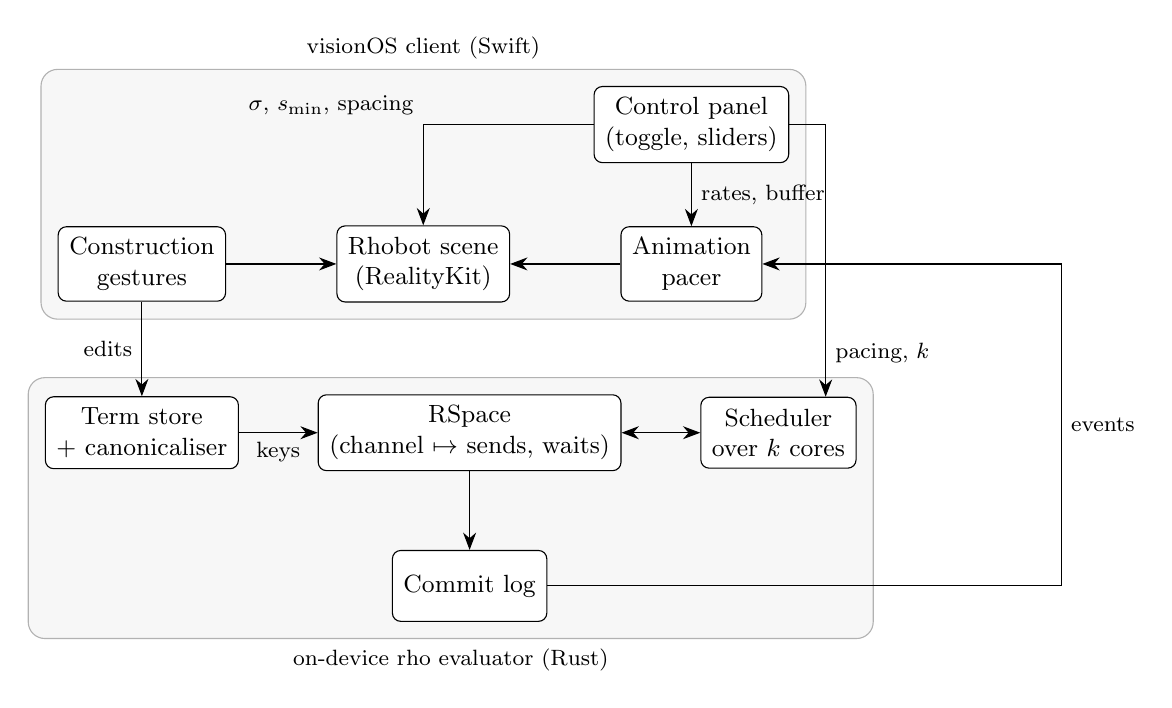
\begin{tikzpicture}[
  box/.style={draw, rounded corners=3pt, align=center, font=\small, minimum height=9mm, inner sep=4pt, fill=white},
  grp/.style={draw=gray!60, rounded corners=6pt, inner sep=6pt, fill=gray!6},
  >={Stealth[length=2.2mm]}]
\node[box] (editor) {Construction\\gestures};
\node[box, right=14mm of editor] (scene) {Rhobot scene\\(RealityKit)};
\node[box, right=14mm of scene] (anim) {Animation\\pacer};
\node[box, above=8mm of anim] (panel) {Control panel\\(toggle, sliders)};
\node[box, below=12mm of editor] (term) {Term store\\+ canonicaliser};
\node[box, right=10mm of term] (rspace) {RSpace\\(channel $\mapsto$ sends, waits)};
\node[box, right=10mm of rspace] (sched) {Scheduler\\over $k$ cores};
\node[box, below=10mm of rspace] (log) {Commit log};
\begin{scope}[on background layer]
  \node[grp, fit=(editor)(scene)(anim)(panel), label={[font=\footnotesize]above:visionOS client (Swift)}] {};
  \node[grp, fit=(term)(rspace)(sched)(log), label={[font=\footnotesize]below:on-device rho evaluator (Rust)}] {};
\end{scope}
\draw[->] (editor) -- (scene);
\draw[->] (editor) -- node[left,font=\footnotesize]{edits} (term);
\draw[->] (term) -- node[below,font=\footnotesize]{keys} (rspace);
\draw[<->] (rspace) -- (sched);
\draw[->] (rspace) -- (log);
\draw[->] (log.east) -- ($(log.east -| sched.east)+(26mm,0)$) |- node[pos=0.25,right,font=\footnotesize]{events} (anim.east);
\draw[->] (anim) -- (scene);
\draw[->] (panel) -- node[right,font=\footnotesize]{rates, buffer} (anim);
\draw[->] (panel.west) -| node[pos=0.5,above left,font=\footnotesize]{$\sigma$, $s_{\min}$, spacing} (scene.north);
\draw[->] (panel.east) -| node[pos=0.92,right,font=\footnotesize]{pacing, $k$} ($(sched.north)+(6mm,0)$);
\end{tikzpicture}
\caption[Runtime components]{Runtime components. The scene edits terms; the evaluator decides and logs
communications; the scene animates the log. The control panel sets rendering parameters,
playback rates, and the pacing mode, which the scheduler enforces as admission control.}
\label{fig:arch}
\end{figure}

\paragraph{Evaluator.} The evaluator is an RSpace over pure rho (Figure~\ref{fig:arch}).
\begin{itemize}
  \item A top-level send \emph{produces} its payload at its channel's canonical key.
  \item A top-level receive \emph{consumes} at its key.
  \item A match commits atomically and yields the continuation with the substitution applied.
  \item Its top-level parallel components are then fed back as new produces and consumes.
  \item Worker threads, $k$ of them as set on the control panel, race on keys under striped locks. The
    scheduler owns thread assignment and commit admission, and is the single place where
    scheduling policy lives. In lockstep mode admission waits for the scene's acknowledgment;
    in free-running mode it does not (\S\ref{sec:pacing}).
\end{itemize}

\paragraph{Relation to \texttt{f1r3node-rust} (\texttt{feature/cost-accounted-rho}).}
The node supplies the reference implementation and possibly reusable parts.
\begin{itemize}
  \item \texttt{rspace++} provides the tuple-space core, matcher and striped locks. Its hot
    store is in memory; its history layer depends on LMDB through \texttt{heed}. Version 1
    needs only the hot store. Building for the visionOS Rust target is to be verified.
  \item The node's \texttt{Par} normal form and sorter provide canonical ordering. Pure rho
    maps into the node's grammar through \texttt{Nil}, \texttt{x!(P)},
    \texttt{for(y <- x)\{P\}}, \texttt{|}, \texttt{*x} and \texttt{@P}. This allows
    differential testing of the on-device evaluator against the node.
  \item The \texttt{rho-pure-eval} crate evaluates guard expressions for \texttt{where}
    clauses. Despite its name it is not a process reducer and is not the evaluator
    described here.
  \item Deployment of a constructed term to a shard, and cost accounting on the scene, are
    deferred.
\end{itemize}

\paragraph{The $\mathsf{stdin}$ channel.} The evaluator reserves one channel key for
$\mathsf{stdin}$. The scene's input gesture becomes a produce on that key, carrying the quoted
process the programmer placed. For differential testing against the node, $\mathsf{stdin}$
corresponds to a system channel rather than to any quoted process.

\paragraph{Transport.} Version 1 runs the evaluator in-process on the headset, linked as a
static library behind a C ABI. This avoids the device-boundary transport failures met during
the F1R3Skein bring-up.

%======================================================================
\section{Reserved vocabulary for f1r3lang}\label{sec:reserved}

\begin{table}[h]
\centering\small
\begin{tabularx}{\linewidth}{@{}l X@{}}
\toprule
f1r3lang construct & Reserved rhobot form\\
\midrule
Patterns in receipts & The binder platform takes the shape of the pattern: a moulded tray
  with sub-platforms for pattern variables.\\
Joins (\texttt{;} and \texttt{\&}) & One waiting robot with several appendages, one per
  receipt; all hands must be served for the robot to commit.\\
\texttt{where} clauses & A visor on the waiting robot through which payloads are inspected
  before acceptance.\\
Graded \texttt{where} & The visor shows a meter; the value in the resolution algebra
  decorates the commit.\\
\texttt{new} & An enclosure on the plane; channels minted inside carry an unforgeable
  fingerprint.\\
Ground values & Tokens rather than robots, carried in capsules.\\
DDL \texttt{Theory} terms & Distinct robot species per theory, with rewrites as a second
  kind of animation.\\
Cost accounting & A charge gauge on each robot, drawn down by the commits it takes part in.\\
\bottomrule
\end{tabularx}
\end{table}

\end{document}
